\addcontentsline{toc}{chapter}{Introduction}
From the begining of computing, the machines have solve probems incredibly difficult for a human, problems based on mathematicals rules. But what has been a really difficult task for computer was to solve some problems that are simple and easy for humans such as images or speech recognition. Tasks that a person perform easily but that are difficult to describe formally.

A person needs a big amount of knowledge to live and to understand, and many times this knowledge cannot be described in a formal way. That means that if we want the computers to performs the same tasks as an human, that computer should acquire that knowledge, by learning.\\

If it is said that a computer learns that means that it understands a complex concept as a hierachy of simpler concepts. The hierachy of concepts is deep, with many layers composed of concepts, and hence the term of deep learning.\\

To achieve this approach Neural Networks are going to be used. They are copying the behaviour of a brain neural network. Multiple layers of neurons that are connected to each others and pass information through those connections. This model, allows the computer to learn since the neurons adapt the output for a given input depending on the expected answer. That means that with a big amount of data to learn, the network could predict a correct answer for the input. \cite{deepbook}

\chapter{Neural Networks}
The brain has been studied deeply during the last century. The researchers wanted to use the power of the brain in a mathematical or computational model. The first step in the Deep Learning was to copy the behaviour of the brain neurons to a circuit (1943, neurophysiologist Warren McCulloch and mathematician Walter Pitts). The poor computing capacity of the time stopped the studies on the topic.\\

In the 80s the field became again interesting with the inclusion of multiple layered neural networks. In 1986 researchers modeled the idea of back propagation. This idea helps the network to distribute pattern recognition errors throughout the whole network. The problem is that with this algorithm the net learn slowly, so many iterations are needed. \\

Nowadays Neural Networks are incredibly important. The big data and the computing capacity are a perfect base for the networks. Also with new types of models such as Convolutional Neural Networks or Recurrent Neural Networks they are solving amazing problems beyond the image recognition. \cite{hnet1} \cite{hnet2}

\section{What is a Neural Network}
You could think of a Neural Network as a box with a certain number of inputs and outputs. For a given input the box answer with a output, that is the network prediction.

Let us imagine that we have one box of this kind, and if you input a image of a handwritten digit, the output of the box will be the digit of the picture. You could think that if you create one box like this you have all your work done, but the box by itself is stupid. If you create a box and feed it with the picture of a '1' the output could be whatever.

What we should do is to teach the net so it could answer correctly. To achieve it our box has several knobs that we can regulate in order to tell the box how bad was the prediction it said. In that way, after correcting the knobs several times, the box has learned, what means that it is ready for answer right. Now we have a box with the knowledge to make good predictions, but since it is a box we cannot outcome any knowledge for us. We cannot get any method to create an algorythm that solve our task more efficiently. We just can use our box, and get our answer from our box.

\subsection{Under the Hood}
Now that we have understood our box it is time to start knowing what is inside it. The neural network is composed by several layers. At least we have the input layer (receive the data from outside) and the output layer (give us the prediction). Between those two could be more hidden layers. Each of them has a certain number of neurons $n_1, n_2, .., n_m$ where $m$ is the number of layers. That means that the input layer has $n_1$ neurons while the output layer has $n_m$ neurons. Each neuron of the first layer is connected with each neuron of the second layer, each neuron of the second layer is connected with each neuron of the third layer and so on (See Figure ~\ref{fig:net2}). \\

\begin{figure}
  \center
  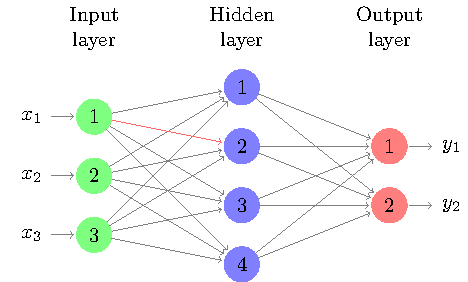
\includegraphics[scale=1.5]{images/net2.pdf}
  \caption{\label{fig:net2}Example of Neural Network with 3 layers. Here $n_1=3$, $n_2=4$ and $n_3=2$. The connection in red is denoted as $w^{(1)}_{12}$ (according to Equation ~\ref{eq:w})}
\end{figure}

Each of those connections has a weight $w$. To denote these weights we are going to use the form $w_{ij}^{(k)}$ where $k$ means which layer the connection departs from, $i$ means which neuron of layer $k$ the connection departs from and $j$ means which neuron of layer $k+1$ the connections arrives to (See Figure ~\ref{fig:net2}). Therefore $w$ is:
\begin{equation}
\begin{aligned}
  & w^{(k)}_{ij} \\
  & i=1,\dots,n_k \\
  & j=1,\dots,n_{k+1} \\
  & k=1,\dots,m
\end{aligned}
\label{eq:w}
\end{equation}\\

Each neuron has a bias that allow set how excited is a neuron. A really excited neuron always output '1' while a non-excited neuron always give us '0'. The bias helps the network to adjust some neurons as important since not every neuron output is equally interesting. The work of a single neuron is as simple as add the bias and the weighted inputs and apply a function to the result ~\cite[Chapter~27]{springer}. The output $o$ of a neuron is:
\begin{equation}
  o^{(k)}_i=f\bigg(u^{(k)}_i+\sum^{n_{k-1}}_{j=1}w^{(k-1)}_{ji}\cdot o^{(k-1)}_j\bigg)
\end{equation}
The output of the input layer is just $o^{(0)}_i=x_i$ since there is not any output before. For example, for the neuron 3 in blue of Figure ~\ref{fig:net2} the output will be $o^{(2)}_3=f(u^{(2)}_3+w^{(1)}_{13}\cdot o^{(1)}_1+w^{(1)}_{23}\cdot o^{(1)}_2+w^{(1)}_{33}\cdot o^{(1)}_3)$. For the same neuron the scheme is showed in Figure ~\ref{fig:neur1}.
\begin{figure}
  \center
  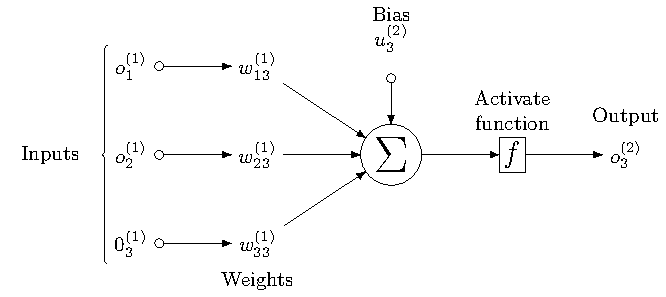
\includegraphics[scale=1]{images/neuron1.pdf}
  \caption{\label{fig:neur1}Example of the task of a single neuron \cite{neurdiag}}
\end{figure}
